% !TEX encoding = UTF-8
% !TEX program = pdflatex
% !TEX root = InformationRetrieval.tex
% !TEX spellcheck = it-IT

% 1 Dicembre 2016

% \subsection{La dimensione del web}
% continua...

Un primo limite inferiore per la dimensione del web indicizzabile può essere ottenuto andando a considerare l'intersezione degli insiemi di pagine che sono indicizzate dai maggiori motori di ricerca.
Questo calcolo però non è semplice in quanto i vari motori di ricerca non forniscono informazioni riguardo a quali pagine indicizzano.

Un approccio alternativo è quello di generare un'insieme casuale di query da sottoporre ai vari motori di ricerca e selezionare un'insieme di URL dai risultati forniti dai vari motori, assumendo che questo insieme sia un campione uniforme delle pagine indicizzate.
Si possono quindi utilizzare questi URL per andare a testare se i vari motori di ricerca indicizzano quelle pagine.

Così facendo, dati due motori di ricerca $A$ e $B$ possiamo andare a stimare l'intersezione delle pagine che indicizzano.

Si può quindi stimare la probabilità che un URL presente in un motore di ricerca $A$ sia contenuto anche nell'intersezione:

$$
P(A \cap B | A) = \frac{\text{Numero di URL nell'intersezione}}{\text{numero di URL in }A}
$$

Inoltre, se è nota la dimensione di $A$ si può anche stimare la dimensione dell'intersezione e di $B$:

$$
|A \cap B| = |A| \cdot P(A \cap B | A) \quad \text{e} \quad |B| = \frac{|A \cap B|}{P(A \cap B | B)}
$$

e di conseguenza ottenere anche la dimensione dell'unione.

Tutto questo può essere utile per comparare l'indice del proprio motore di ricerca con altri già esistenti.


\section{I meta tag delle pagine}

All'interno del head di una pagina web è possibile andare a specificare delle informazioni riguardanti il contenuto e l'autore della pagina che rimangono nascoste all'utente finale.

Con la sempre più ampia diffusione dei motori di ricerca e data la necessità di fornire sempre risultati migliori, si è reso necessario estendere questo meccanismo dei meta-tag arrivando al cosiddetto web semantico.

In pratica sono stati definiti degli schemi standard di tag da utilizzare all'interno delle pagine per indicare le informazioni relative ai contenuti delle pagine.
Il più famoso di questi schemi è il \textbf{dublin core}.

Tra i tag definiti nel dublin core ci sono quelli per definire l'autore della pagina, la data dell'ultima modifica 

\section{Le interrogazioni nel web}

Tipicamente le query web sono composte da poche parole, mediamente 2 o 3, e gli argomenti sono molto generici.

Fino a poco tempo, come modello di riferimento veniva utilizzato un modello booleano che metteva in \textit{and} tutti i termini presenti nella query. I documenti trovati venivano poi ordinati i risultati per rilevanza.
Tuttavia in questo ultimo periodo la prima parte è stata rilassata: non viene più effettuato un exact-match, ma vengono presi in considerazione anche i sinonimi. Inoltre, nel ranking viene tenuto conto anche della rete sociale e dello storico dell'utente.

Si ha inoltre che la distribuzione delle query effettuate dall'utente ha una coda lunga, ovvero ci sono poche query che vengono effettuate molto frequentemente e tante query che vengono effettuate raramente.

\begin{figure}[htbp]
	\centering
	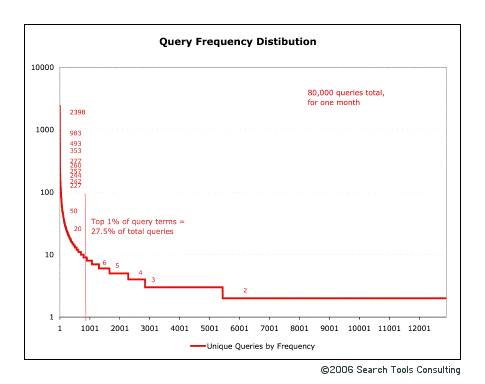
\includegraphics[width=.6\textwidth]{images/l18-fig-1.png}
\end{figure}

Anche il periodo/luogo influisce nella popolarità di un query. Vedi l'esempio della frequenza dei termini \textit{Monti-Letta-Renzi} oppure della query \textit{terremoto} che è più frequente nelle regioni dell'Italia centrale.

Le query possono essere divise in 3 categorie:

\begin{itemize}
	\item \textbf{Di navigazione}: l'utente vuole localizzare una specifica pagina o sito web. Solitamente la query ha un unico risultato corretto che è una pagina del sito che l'utente cerca. I risultati potrebbero essere localizzati in base alla regione dell'utente, ad esempio fornendo il sito scritto nella lingua del paese dal quale proviene la query.
	\item \textbf{Informativa}: l'utente è interessato a conoscere qualcosa su uno specifico argomento. In questo caso non è importante chi quale sia la sorgente, l'importante è che questa sia affidabile. Anche in questo caso si può profilare l'utente per mettere in evidenza le pagine che si ritiene che possano interessare all'utente.
	\item \textbf{Transazionale}: l'utente è interessato a trovare un sito per poi utilizzarlo per acquistare dei prodotti. \`E simile alla prima categoria.
\end{itemize}

\section{Web Crawler}

Un web crawler o agente web è un programma che attraversa automaticamente la struttura ipertestuale del web, al fine di recuperare le pagine da indicizzare.
\`E compito del web crawler analizzare i meta-tag per stabilire se una determinata pagina è interessante o meno per il nostro indice che stiamo costruendo. Il crawler si comporta quindi come l'ente che fornisce la collezione da indicizzare.

\begin{figure}[htbp]
	\centering
	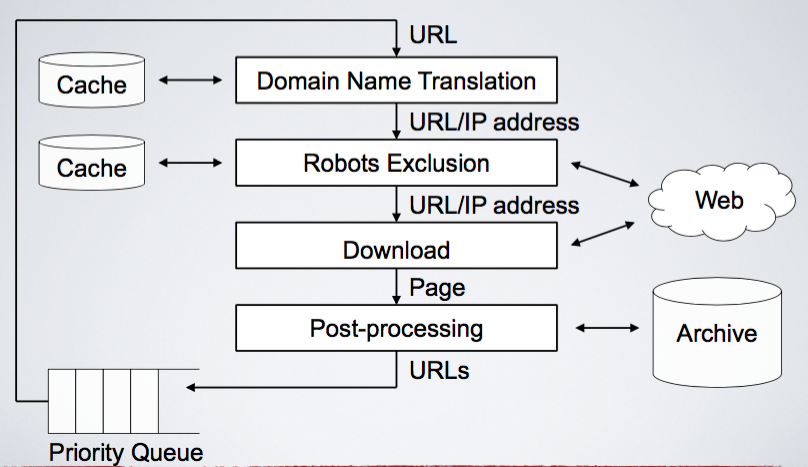
\includegraphics[width=.6\textwidth]{images/l18-fig-2.png}
\end{figure}


Il crawler ha bisogno di alcuni URL di partenza che prende il nome di \textbf{lista di seed}, la quale definisce una serie di URL e le politiche di visita degli indirizzi.
Ad esempio si può configurare il crawler in modo che visiti solamente le pagine presenti su alcuni domini.

\`E necessario poi andare a tradurre l'URL in un IP mediante un servizio DNS o una chace. Una volta fatto ciò si può richiedere la pagina web al server, tenendo però conto del file \texttt{robot.txt} il quale contiene la descrizione dei vincoli per l'indicizzazione del contenuto del sito (\textbf{robot esclusion}).
\`E buona norma rispettare le restrizioni, perché altrimenti il server potrebbe bloccare del tutto l'accesso al robot.

Quindi solo se le limitazioni lo consentono vengono scaricate le pagine web per essere analizzate e processate. Durante l'analisi vengono estratti altri URL che il web crawler visiterà oltre ai seed, secondo un certa coda di priorità.
La profondità di visita dei siti web può essere un parametro stabilito dal progettatore del crawler oppure può essere specificata nel file \texttt{robot.txt} del sito.

Sempre nello stesso file è possibile trovare una limitazione temporale all'intervallo di richiesta delle pagine al server, ad esempio una richiesta ogni 5 secondi, questo per evitare di sovraccaricare il server e intralciare la navigazione degli utenti normali.

\textbf{{\color{Red} Possibile esercizio:}} Si definisca che cosa è un agente web; si descrivano i componenti e i compiti di un Web Crawler.


















